\chapter{Results}

\section{Simulated Data}

\subsection{Test Cases}

The test cases looked at were selected to determine the effects of the spacecraft inertia, the spacecrafts orbit and its geometry. In Total 18 total cases were simulated, each at multiple different time of the year and multiple random angular velocities.

The geometries used in this analysis were a rectangular prism, a cylinder, and a box-wing. The first two are convex geometries that have differing levels of symmetry, while the box-wing geometry is concave. The orbits examined are low, medium and geostationary Earth orbits. The final variable is the spacecrafts inertia. In the first case, the pricipal inertial axes are assumed to be aligned with the spacecraft body frame and equal. The effect of this is to make the spin axis constant for all time. In the second case, the principal inertial axes are all different and are not aligned with the body frame, causing the spin axis to change over time.

\begin{figure}
	\begin{tabular}{cc}
		\includegraphics[width = 65mm]{Long_Rectangle_Image.png} &
		\includegraphics[width=65mm]{Cylinder_Image} \\
		Rectangular Prism & Cylinder \\
		\multicolumn{2}{c}{\includegraphics[width=65mm]{Box_Wing_Image}} \\
		\multicolumn{2}{c}{Box Wing}
	\end{tabular}
	\caption{Three Simulated Geometries.}
\end{figure}


\begin{figure}
	\begin{tabular}{cc}
		\includegraphics[width = 65mm]{leo_orbit} &
		\includegraphics[width=65mm]{meo_orbit} \\
		Low Earth Orbit & Medium Earth Orbit \\
		\multicolumn{2}{c}{\includegraphics[width=65mm]{geo_orbit}} \\
		\multicolumn{2}{c}{Geostationary Orbit}
	\end{tabular}
	\caption{Three Simulated Orbits.}
\end{figure}

\subsection{Simulation Methodology}

First, a LEO, MEO, and GEO orbit were selected. Passes were calculated by brute force sampling a spacecrafts location and checking for necessary conditions. These conditions were obviously that the spacecraft must be above the horizon of the observation site and that the spacecraft be illuminated. Passes lower than 20 degrees elevation were discarded. Additionally, in preliminary experiments it was noticed that the UKF often failed to converge to a solution when the solar phase angle (SPA) was greater than 90 degrees. Therefore passes with an SPA greater than 90 degrees were also discarded. Passes were also limited to only 5 minutes of data collection as MEO spacecraft passes can be hours long and geostationary passes are of course perpetual.

Once a pass was identified, the spacecraft was given three initial attitudes and angular velocities between 0.1 and 0.3 radians per second. These were then propagated and used to calculate three different light curves per pass. Before entering the Kalman Filter, Gaussian noise was added to the light curve whose distribution was similar to that of the real data collected.
\subsection{Simulation Results}

The simulation results reveal that the problem of uniquely identifying an attitude profile from a light curve is an indeterminate problem. The data shows that for any light curve, there are multiple attitude profiles that can produce it.

\section{Real Data}

\subsection{SERT-2}

The Space Electric Rocket Test II (SERT-2) is a modified Aegena rocket body whose mission was to test two ion propulsion systems on board. \cite{sert2} In order to power these propulsion systems, two deployable solar panels were added to the Aegena rocket body whose dimensions were 1.5x6 meters. The dimensions of the Aegena module were also 1.53x6 meters.

SERT-2 was launched on February 3rd, 1970 and was finally decommissioned in 1991. Due to the age of the spacecraft and considering that there is potentially fuel remaining within the Aegena tank, this spacecraft can be assumed to be spinning about its major axis. This obviously simplifies the UKF model and allows this thesis to implement the simpler version.

The geometry of SERT-2 is essentially a cylinder with two rectangular panels radiating from one end. This model is non-convex which means that it can take advantage of ray tracing algorithm described in this thesis. 

\begin{figure}
	\centering
	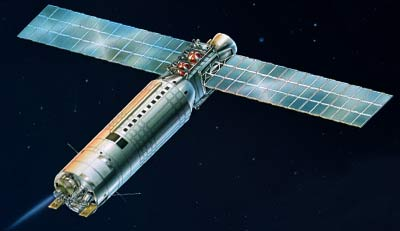
\includegraphics[width = 80mm]{figures/sert-2}
	\caption{SERT-2, Source: NASA}
\end{figure}


\subsection{Ajisai (EGS)}

Ajisai was a mission launched on August 13th, 1986 and was primarily intended as a dummy payload for the H-I launch vehicle. \cite{ajisai_jaxa} Ajisai is essentially a sphere covered with 1,436 corner cube reflectors and 318 mirrors. \cite{ajisai} Its secondary mission (after being mass) was to determine the exact position of the more isolated Japanese islands. \cite{ajisai_jaxa}

Because this spacecraft is so old and because it is a sphere. It is highly likely that it is spinning about its major axis and the simpler UKF formulation can be applied once more.

\begin{figure}
	\centering
	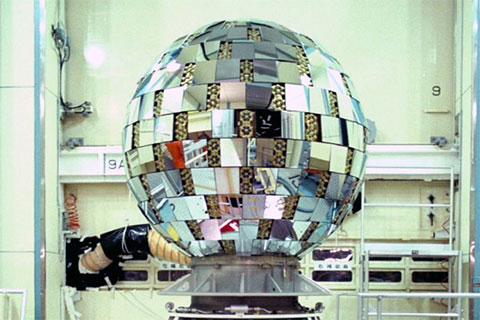
\includegraphics[width = 80mm]{figures/ajisai.jpg}
	\caption{Ajisai, Source: JAXA}
\end{figure}

The geometry of the spacecraft is simply a large set of reflective panels. Being mirrors, these panels will have very high specular reflectance and almost no diffuse reflectance. The corner cube reflectors designed to reflect light back to its source. For this thesis, that source is the sun, and so the corner cube reflectors can be assumed to contribute nothing to the lightcurve. Thankfully, the positions of each corner cube reflector were documented, and the panel locations can be inferred from them.

\begin{figure}
	\centering
	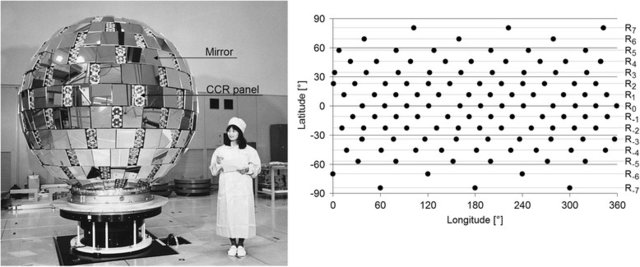
\includegraphics[width = 150mm]{figures/ajisai_panels.jpg}
	\caption{Ajisai with Engineer [Left]. Corner Cube Reflector Locations [Right] \cite{ajisai}}
\end{figure}

\section{Symmetrical Solution Groups}